% Options for packages loaded elsewhere
\PassOptionsToPackage{unicode}{hyperref}
\PassOptionsToPackage{hyphens}{url}
%
\documentclass[
]{article}
\usepackage{lmodern}
\usepackage{amssymb,amsmath}
\usepackage{ifxetex,ifluatex}
\ifnum 0\ifxetex 1\fi\ifluatex 1\fi=0 % if pdftex
  \usepackage[T1]{fontenc}
  \usepackage[utf8]{inputenc}
  \usepackage{textcomp} % provide euro and other symbols
\else % if luatex or xetex
  \usepackage{unicode-math}
  \defaultfontfeatures{Scale=MatchLowercase}
  \defaultfontfeatures[\rmfamily]{Ligatures=TeX,Scale=1}
\fi
% Use upquote if available, for straight quotes in verbatim environments
\IfFileExists{upquote.sty}{\usepackage{upquote}}{}
\IfFileExists{microtype.sty}{% use microtype if available
  \usepackage[]{microtype}
  \UseMicrotypeSet[protrusion]{basicmath} % disable protrusion for tt fonts
}{}
\makeatletter
\@ifundefined{KOMAClassName}{% if non-KOMA class
  \IfFileExists{parskip.sty}{%
    \usepackage{parskip}
  }{% else
    \setlength{\parindent}{0pt}
    \setlength{\parskip}{6pt plus 2pt minus 1pt}}
}{% if KOMA class
  \KOMAoptions{parskip=half}}
\makeatother
\usepackage{xcolor}
\IfFileExists{xurl.sty}{\usepackage{xurl}}{} % add URL line breaks if available
\IfFileExists{bookmark.sty}{\usepackage{bookmark}}{\usepackage{hyperref}}
\hypersetup{
  pdftitle={Resumo de Programação C},
  pdfauthor={Paulino Ng},
  hidelinks,
  pdfcreator={LaTeX via pandoc}}
\urlstyle{same} % disable monospaced font for URLs
\usepackage{color}
\usepackage{fancyvrb}
\newcommand{\VerbBar}{|}
\newcommand{\VERB}{\Verb[commandchars=\\\{\}]}
\DefineVerbatimEnvironment{Highlighting}{Verbatim}{commandchars=\\\{\}}
% Add ',fontsize=\small' for more characters per line
\newenvironment{Shaded}{}{}
\newcommand{\AlertTok}[1]{\textcolor[rgb]{1.00,0.00,0.00}{\textbf{#1}}}
\newcommand{\AnnotationTok}[1]{\textcolor[rgb]{0.38,0.63,0.69}{\textbf{\textit{#1}}}}
\newcommand{\AttributeTok}[1]{\textcolor[rgb]{0.49,0.56,0.16}{#1}}
\newcommand{\BaseNTok}[1]{\textcolor[rgb]{0.25,0.63,0.44}{#1}}
\newcommand{\BuiltInTok}[1]{#1}
\newcommand{\CharTok}[1]{\textcolor[rgb]{0.25,0.44,0.63}{#1}}
\newcommand{\CommentTok}[1]{\textcolor[rgb]{0.38,0.63,0.69}{\textit{#1}}}
\newcommand{\CommentVarTok}[1]{\textcolor[rgb]{0.38,0.63,0.69}{\textbf{\textit{#1}}}}
\newcommand{\ConstantTok}[1]{\textcolor[rgb]{0.53,0.00,0.00}{#1}}
\newcommand{\ControlFlowTok}[1]{\textcolor[rgb]{0.00,0.44,0.13}{\textbf{#1}}}
\newcommand{\DataTypeTok}[1]{\textcolor[rgb]{0.56,0.13,0.00}{#1}}
\newcommand{\DecValTok}[1]{\textcolor[rgb]{0.25,0.63,0.44}{#1}}
\newcommand{\DocumentationTok}[1]{\textcolor[rgb]{0.73,0.13,0.13}{\textit{#1}}}
\newcommand{\ErrorTok}[1]{\textcolor[rgb]{1.00,0.00,0.00}{\textbf{#1}}}
\newcommand{\ExtensionTok}[1]{#1}
\newcommand{\FloatTok}[1]{\textcolor[rgb]{0.25,0.63,0.44}{#1}}
\newcommand{\FunctionTok}[1]{\textcolor[rgb]{0.02,0.16,0.49}{#1}}
\newcommand{\ImportTok}[1]{#1}
\newcommand{\InformationTok}[1]{\textcolor[rgb]{0.38,0.63,0.69}{\textbf{\textit{#1}}}}
\newcommand{\KeywordTok}[1]{\textcolor[rgb]{0.00,0.44,0.13}{\textbf{#1}}}
\newcommand{\NormalTok}[1]{#1}
\newcommand{\OperatorTok}[1]{\textcolor[rgb]{0.40,0.40,0.40}{#1}}
\newcommand{\OtherTok}[1]{\textcolor[rgb]{0.00,0.44,0.13}{#1}}
\newcommand{\PreprocessorTok}[1]{\textcolor[rgb]{0.74,0.48,0.00}{#1}}
\newcommand{\RegionMarkerTok}[1]{#1}
\newcommand{\SpecialCharTok}[1]{\textcolor[rgb]{0.25,0.44,0.63}{#1}}
\newcommand{\SpecialStringTok}[1]{\textcolor[rgb]{0.73,0.40,0.53}{#1}}
\newcommand{\StringTok}[1]{\textcolor[rgb]{0.25,0.44,0.63}{#1}}
\newcommand{\VariableTok}[1]{\textcolor[rgb]{0.10,0.09,0.49}{#1}}
\newcommand{\VerbatimStringTok}[1]{\textcolor[rgb]{0.25,0.44,0.63}{#1}}
\newcommand{\WarningTok}[1]{\textcolor[rgb]{0.38,0.63,0.69}{\textbf{\textit{#1}}}}
\usepackage{longtable,booktabs}
% Correct order of tables after \paragraph or \subparagraph
\usepackage{etoolbox}
\makeatletter
\patchcmd\longtable{\par}{\if@noskipsec\mbox{}\fi\par}{}{}
\makeatother
% Allow footnotes in longtable head/foot
\IfFileExists{footnotehyper.sty}{\usepackage{footnotehyper}}{\usepackage{footnote}}
\makesavenoteenv{longtable}
\usepackage{graphicx,grffile}
\makeatletter
\def\maxwidth{\ifdim\Gin@nat@width>\linewidth\linewidth\else\Gin@nat@width\fi}
\def\maxheight{\ifdim\Gin@nat@height>\textheight\textheight\else\Gin@nat@height\fi}
\makeatother
% Scale images if necessary, so that they will not overflow the page
% margins by default, and it is still possible to overwrite the defaults
% using explicit options in \includegraphics[width, height, ...]{}
\setkeys{Gin}{width=\maxwidth,height=\maxheight,keepaspectratio}
% Set default figure placement to htbp
\makeatletter
\def\fps@figure{htbp}
\makeatother
\setlength{\emergencystretch}{3em} % prevent overfull lines
\providecommand{\tightlist}{%
  \setlength{\itemsep}{0pt}\setlength{\parskip}{0pt}}
\setcounter{secnumdepth}{-\maxdimen} % remove section numbering

\title{Resumo de Programação C}
\author{Paulino Ng}
\date{2019-09-30}

\begin{document}
\maketitle

\begin{quote}
Advertência: Este é um trabalho em andamento (WIP - work-in-progress).
\end{quote}

\hypertarget{programa-alo}{%
\subsection{Programa Alo}\label{programa-alo}}

Seguindo os passos de {[}1{]}, este resumo começa com o programa alo.c,
cujo código é:

\begin{Shaded}
\begin{Highlighting}[]
\PreprocessorTok{#include }\ImportTok{<stdio.h>}

\DataTypeTok{int}\NormalTok{ main() \{}
\NormalTok{  printf(}\StringTok{"Alo!}\SpecialCharTok{\textbackslash{}n}\StringTok{"}\NormalTok{);}
  \ControlFlowTok{return} \DecValTok{0}\NormalTok{;}
\NormalTok{\}}
\end{Highlighting}
\end{Shaded}

A linha \texttt{\#include\ \textless{}stdio.h\textgreater{}} pede para o
pré-compilador do C incluir o arquivo \texttt{stdio.h} no lugar da
linha. Isto permite usar a chamada da função \texttt{printf()}.

Todo programa C deve ter uma implementação da função \texttt{main()}.
Esta é a função que o sistema operacional \emph{chama} ao carregar o
programa para a execução.

A função \texttt{main()} retorna um valor inteiro para indicar se o
programa executou corretamente ou não. Se a \texttt{main()} retorna
\texttt{0} (zero), o programa executou sem erros. Se executar com algum
tipo de erro, o valor do retorno é diferente de \texttt{0}.

Além da instrução de retorno, a única instrução dentro do corpo da
\texttt{main()} é a chamada à função \texttt{printf()}. A função
\texttt{printf()} imprime uma mensagem (\emph{texto}) na tela do usuário
(na \emph{console} do usuário). A mensagem é o argumento da chamada da
função, \texttt{"Alo!\textbackslash{}n"}. Este texto é chamado de
\emph{string} e consiste na sequência de caracteres
\texttt{\textquotesingle{}A\textquotesingle{}},
\texttt{\textquotesingle{}l\textquotesingle{}},
\texttt{\textquotesingle{}o\textquotesingle{}},
\texttt{\textquotesingle{}!\textquotesingle{}},
\texttt{\textquotesingle{}\textbackslash{}n\textquotesingle{}} e
\texttt{\textquotesingle{}\textbackslash{}0\textquotesingle{}}. O
carácter \texttt{\textquotesingle{}\textbackslash{}n\textquotesingle{}}
é para terminar a linha do \texttt{"Alo!"} e começar um nova.

As instruções em C terminam com um \texttt{;} obrigatório.

\hypertarget{etapas-para-a-gerauxe7uxe3o-de-um-programa-executuxe1vel-de-c}{%
\subsection{Etapas para a geração de um programa executável de
C}\label{etapas-para-a-gerauxe7uxe3o-de-um-programa-executuxe1vel-de-c}}

\begin{figure}
\centering
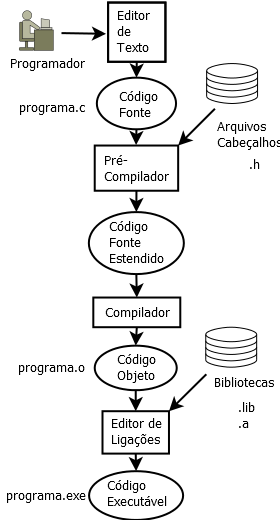
\includegraphics{images/etapas_compilacao.png}
\caption{Etapas da edição até o código executável.}
\end{figure}

O C é uma linguagem de programação compilada. Isto é, o código fonte
precisa ser compilado para poder ser executado, diferente de linguagem
interpretada cujos programas não precisam ser compilados para serem
executados pelo interpretador. Como ocorre com o Python.

A figura ilustra o código fonte que é inicialmente editado pelo
programador com o uso de um \emph{editor de texto}. Isto resulta num
arquivo \texttt{.c}. Este arquivo é processado pelo pré-compilador que
inclui os arquivos cabeçalhos, substitui as macros, \ldots{} Isto gera
um arquivo intermediário que é compilado pelo \emph{compilador}. O
arquivo compilado é um código objeto, ou arquivo objeto. Este arquivo é
binário e já possui as instruções de máquina da tradução das instruções
C do código fonte. Este código, entretanto ainda não pode ser executado,
pois falta o código das bibliotecas. O \emph{editor de ligações} é quem
\emph{costura} o código objeto com as bibliotecas e constrói o
\emph{arquivo executável}.

Os sistemas operacionais modernos trabalham com bibliotecas
compartilhadas, isto é, bibliotecas cujas funções podem ser
compartilhadas entre diferentes aplicações durante a execução. Assim, o
código executável pode não ter todas as instruções que o programa
precisa para ser executado. Se uma função de uma biblioteca
compartilhada (\texttt{.dll}) for necessária para um programa, o SO se
encarrega de mapeá-la na memória do programa dinamicamente.

\hypertarget{pruxe9-compilador}{%
\subsection{Pré-compilador}\label{pruxe9-compilador}}

\hypertarget{include}{%
\subsubsection{\texorpdfstring{\texttt{\#include}}{\#include}}\label{include}}

Pelo fato do C ser uma linguagem de programação bastante simples, não
existe muita coisa pronta na linguagem. Por outro lado, o C possui uma
grande quantidade de bibliotecas de funções que podem ser reutilizadas
nos programas poupando muito esforço de programação.

As bibliotecas estáticas e dinâmicas estão em arquivos com extensão
\texttt{.a} ou \texttt{.so} no Unix, ou \texttt{.lib} ou \texttt{.dll}
no MS Windows. O editor de ligações estáticas ou dinâmicas vai incluir o
código destas funções ao código executável, mas, antes disto, o
compilador precisa conhecer o protótipo das funções antes das funções
serem chamadas nos programas dos programadores-usuários das bibliotecas.

Esta é uma das funções dos arquivos cabeçalho, fornecer os protótipos
das funções das bibliotecas. Além disso, é nos arquivos cabeçalhos onde
estruturas de dados, constantes e variáveis globais são declaradas em
programas C.

Os arquivos cabeçalho de C, geralmente, usam a extensão \texttt{.h}. Os
arquivos cabeçalho das bibliotecas costumam está em diretórios do
sistema de compilação. Mas, o programador pode criar seus próprios
arquivos cabeçalho e colocá-los em qualquer diretório.

Como as declarações dos arquivos cabeçalho são necessárias para poder
usar as bibliotecas, o programador teria de copiá-los em cada arquivo de
código que utilizasse as funções das bibliotecas. Para evitar estas
cópias, os arquivos de códigos C (tanto código fonte como cabeçalho),
pedem para um pré-compilador (ou pré-processador) para incluir os
arquivos cabeçalho. A instrução
\texttt{\#include\ \textless{}stdio.h\textgreater{}} é uma instrução
para o pré-compilador de C substituir esta linha pelo conteúdo do
arquivo \texttt{stdio.h}. Os \texttt{\textless{}\textgreater{}} servem
para indicar que o arquivo deve ser procurado nos diretórios de sistema.
No lugar de \texttt{\textless{}\textgreater{}} (\emph{bicudos}), podemos
usar \texttt{""}. Isto é, \texttt{\#include\ "stdio.h"}, neste caso, o
pré-compilador procura o arquivo \texttt{stdio.h} no diretório do código
fonte antes dos diretórios de sistema.

\hypertarget{define}{%
\subsubsection{\texorpdfstring{\texttt{\#define}}{\#define}}\label{define}}

Além da instrução \texttt{\#include}, o pré-compilador C permite criar
\emph{macros}. Na sua forma mais simples \emph{macros} servem para
definir constantes. Por exemplo, para definir a constante \(\pi\) em C,
pode-se fazer:

\begin{verbatim}
#define PI 3.141592653589793
\end{verbatim}

Se dentro do código C aparecer o nome da \emph{macro} (\texttt{PI}), o
nome vai ser substituído pelo valor associado. Por exemplo:

\begin{Shaded}
\begin{Highlighting}[]
\NormalTok{    printf(}\StringTok{"%f"}\NormalTok{, sin(PI/}\DecValTok{4}\NormalTok{));}
\end{Highlighting}
\end{Shaded}

O pré-compilador vai substituir \texttt{PI} pelo valor e o código que
será compilado é:

\begin{Shaded}
\begin{Highlighting}[]
\NormalTok{    printf(}\StringTok{"%f"}\NormalTok{, sin(}\FloatTok{3.141592653589793}\NormalTok{/}\DecValTok{4}\NormalTok{));}
\end{Highlighting}
\end{Shaded}

Mas \emph{macro} é um mecanismo geral, o nome da macro pode ser
substituído por qualquer texto de programa. Assim, se quisermos usar a
palavra \texttt{Enquanto} no lugar de \texttt{while}, poderíamos criar a
macro:

\begin{Shaded}
\begin{Highlighting}[]
\PreprocessorTok{#define Enquanto while}
\end{Highlighting}
\end{Shaded}

E escrever o código com:

\begin{Shaded}
\begin{Highlighting}[]
\DataTypeTok{int}\NormalTok{ main() \{}
  \DataTypeTok{int}\NormalTok{ i = }\DecValTok{0}\NormalTok{;}
\NormalTok{  Enquanto (i < }\DecValTok{10}\NormalTok{) \{}
\NormalTok{    printf(}\StringTok{"Alo}\SpecialCharTok{\textbackslash{}n}\StringTok{"}\NormalTok{);}
\NormalTok{    i++;}
\NormalTok{  \}}
\NormalTok{\}}
\end{Highlighting}
\end{Shaded}

As macros podem ser parametrizadas, isto é, podemos colocar parâmetros
para as macros. Podemos trocar o \texttt{printf()} do código anterior
para \texttt{Imprima()} com:

\begin{Shaded}
\begin{Highlighting}[]
\PreprocessorTok{#define Imprima(msg) printf(msg)}
\end{Highlighting}
\end{Shaded}

E o código ficaria:

\begin{Shaded}
\begin{Highlighting}[]
\DataTypeTok{int}\NormalTok{ main() \{}
  \DataTypeTok{int}\NormalTok{ i = }\DecValTok{0}\NormalTok{;}
\NormalTok{  Enquanto (i < }\DecValTok{10}\NormalTok{) \{}
\NormalTok{    Imprima(}\StringTok{"Alo}\SpecialCharTok{\textbackslash{}n}\StringTok{"}\NormalTok{);}
\NormalTok{    i++;}
\NormalTok{  \}}
\NormalTok{\}}
\end{Highlighting}
\end{Shaded}

\begin{quote}
Cuidado com \emph{macros}, principalmente as parametrizadas, elas podem
ter efeitos colaterais muito complexos. Elas dificultam a localização e
compreensão de erros de lógica.
\end{quote}

\hypertarget{ifdef-e-ifndef}{%
\subsubsection{\texorpdfstring{\texttt{\#ifdef} e
\texttt{\#ifndef}}{\#ifdef e \#ifndef}}\label{ifdef-e-ifndef}}

Os arquivos cabeçalho incluem outros arquivos cabeçalho e pode ocorrer
de numa sequência de inclusões, um mesmo arquivo ser incluído mais de
uma vez. Imagine que você escreveu um arquivo cabeçalho, \texttt{meu.h},
e por algum motivo seu arquivo cabeçalho precisa da inclusão do arquivo
\texttt{stdlib.h} que possui diversas constantes úteis do sistema. O
código fonte inclui seu arquivo cabeçalho e como também precisa de
algumas constantes do sistema, ele também inclui o arquivo
\texttt{stdlib.h}. Pode ocorrer problemas na compilação se as constantes
forem declaradas múltiplas vezes. Para evitar o erro de múltiplas
declarações (o que não é permitido em C), é necessário usar um esquema
de exclusão de múltiplas declarações. Isto é obtido pelo uso do
condicional do pré-compilador. A estrutura que todos os arquivos de
cabeçalho usam é:

\begin{Shaded}
\begin{Highlighting}[]
\PreprocessorTok{#ifndef _nome_do_arquivo.H_}
\PreprocessorTok{#define _nome_do_arquivo.H_}

\CommentTok{// declarações e outros conteúdos do arquivo cabeçalho}

\PreprocessorTok{#endif}
\end{Highlighting}
\end{Shaded}

Estas instruções para o pré-compilador permitem que um arquivo cabeçalho
seja incluído múltiplas vezes sem provocar dupla declaração de
variáveis, protótipos, etc.

\hypertarget{comentuxe1rios-em-c}{%
\subsection{Comentários em C}\label{comentuxe1rios-em-c}}

Comentários nos códigos fonte são importantes para explicar como usar as
funções e estruturas de dados e para explicar o algoritmo que está sendo
usado para realizar um cálculo. Comentários do tipo:
\texttt{isto\ é\ uma\ variável}, \texttt{esta\ é\ uma\ função},
\texttt{este\ é\ o\ main()}, são inúteis e devem ser evitados.

O C tem 2 tipos de comentários: \texttt{//} e \texttt{/*\ */}.
\texttt{//} inicia um comentário que vai até o final da linha.
\texttt{/*} inicia um comentário que termina quando \texttt{*/} é
encontrado. Isto permite comentários em múltiplas linhas e comentários
no meio de uma linha. Por exemplo:

\begin{Shaded}
\begin{Highlighting}[]
\NormalTok{  x = }\DecValTok{0}\NormalTok{; }\CommentTok{// x é inicializado com 0 (comentário idiota)}
  \CommentTok{/* comentário de várias linhas}
\CommentTok{   * são usados para explicar uso de funções, estruturas de dados e algoritmos.}
\CommentTok{   */}
\NormalTok{  y = }\DecValTok{1}\NormalTok{ + }\CommentTok{/* este é um comentário mal posto */} \DecValTok{41}\NormalTok{;}
\end{Highlighting}
\end{Shaded}

\hypertarget{declarauxe7uxe3o-de-variuxe1veis-em-c}{%
\subsection{Declaração de variáveis em
C}\label{declarauxe7uxe3o-de-variuxe1veis-em-c}}

O C atualmente é uma linguagem fortemente tipada com tipagem estática.
Isto é, todas as variáveis em C precisam ser declaradas antes de serem
utilizadas e o tipo das variáveis não pode mudar durante a execução do
programa. Mas, diferente de algumas linguagens que obrigam as
declarações de variáveis serem feitas no início do arquivo de código
fonte (no caso de variáveis globais), ou no início do corpo das funções
(no caso de variáveis locais), o C permite que as variáveis sejam
declaradas em qualquer posição antes do uso delas (as globais sempre
precisam ser declaradas fora das funções). Alguns programadores gostam
de declarar as variáveis todas no início de um escopo, pois todas as
declarações ficam visíveis no mesmo lugar. Outros preferem declará-las
próximas do seu local de uso. As empresas de SW costumam estabelecer
regras para estas situações nas suas normas de estilo de programação.
Neste resumo, vamos declarar as variáveis globais no início do arquivo
de código fonte ou cabeçalho. As locais serão declaradas próximas ao
local de uso delas.

As variáveis são sempre declaradas com uma das seguintes sintaxes:

\begin{verbatim}
<tipo> nome_da_var;
<tipo> <lista de nomes de variáveis>;
<tipo> nome_da_var = <expressão com valor calculável durante a compilação>;
\end{verbatim}

A seguir, tem-se algumas declarações válidas em C:

\begin{Shaded}
\begin{Highlighting}[]
\DataTypeTok{int}\NormalTok{ x, y, z;       }\CommentTok{// x, y e z são variáveis inteiras (32 bits)}
\NormalTok{log }\DataTypeTok{int}\NormalTok{ lx, ly, lz;    }\CommentTok{// lx, ly e lz são variáveis inteiras (64 bits)}
\DataTypeTok{long}\NormalTok{ lx1;          }\CommentTok{// lx1 é um long int, o int é opcional}
\DataTypeTok{short}\NormalTok{ sx, sy;      }\CommentTok{// sx e sy são inteiros (16 bits)}
\DataTypeTok{float}\NormalTok{ f, g;        }\CommentTok{// f e g são variáveis de ponto flutuante com 32 bits}
\DataTypeTok{double}\NormalTok{ ff, gg;     }\CommentTok{// ff e gg são variáveis de ponto flutuante com 64 bits}
\DataTypeTok{char}\NormalTok{ ch;           }\CommentTok{// ch é uma variável do tipo carácter}
\DataTypeTok{char}\NormalTok{ linha_nova = }\CharTok{'\textbackslash{}n'}\NormalTok{; }\CommentTok{// linha_nova é uma variável do tipo carácter}
                        \CommentTok{// inicializada com \textbackslash{}n}
\DataTypeTok{char}\NormalTok{ nome[}\DecValTok{80}\NormalTok{];          }\CommentTok{// nome é uma variável capaz de guardar 80 caracteres}
\CommentTok{// A seguir declara-se alguns ponteiros, alguns com inicialização}
\DataTypeTok{char}\NormalTok{ *pChNome = }\StringTok{"Joao"}\NormalTok{; }\CommentTok{// pChNome é um ponteiro para o carácter 'J'}
\DataTypeTok{int}\NormalTok{ *pX = &x;      }\CommentTok{// pX é um ponteiro de inteiro para a posição da variável x}
\end{Highlighting}
\end{Shaded}

\hypertarget{funuxe7uxe3o-de-sauxedda-printf}{%
\subsection{\texorpdfstring{Função de saída:
\texttt{printf()}}{Função de saída: printf()}}\label{funuxe7uxe3o-de-sauxedda-printf}}

O \texttt{printf()} da biblioteca \texttt{stdio} do C permite que sejam
enviados textos, \emph{strings}, para a saída padrão (\emph{stdout}),
que, considera-se, é a interface de linha que mandou rodar o programa.

\begin{quote}
Cuidado ao rodar um programa executável do C pela interface gráfica no
MS Windows, ao clicar duas vezes no executável, o programa provoca a
execução de uma janela de \emph{Prompt do DOS}, roda o programa nela,
imprime as saídas nela e, se não estiver programada nenhuma interação
com o usuário, ao terminar a execução, a janela \emph{DOS} é fechada sem
que se tenha tempo para ver as saídas.
\end{quote}

Para usar o \texttt{printf()} é necessário que a instrução
\texttt{\#include\ \textless{}stdio.h\textgreater{}} tenha sido dada no
início do arquivo de código fonte. O protótipo da \texttt{printf()} é:

\begin{verbatim}
int printf(const char *format, ...);
\end{verbatim}

Os \texttt{...} significam lista de valores que podem ser calculados de
expressões, este valores serão \textbf{convertidos} em texto, pelos
conversores expressos na \emph{string} \texttt{format}. \texttt{format}
é uma \emph{string} que tem o texto de saída e embutido neste texto,
existem \emph{posições} onde os valores convertidos para texto devem ser
inseridos. Alguns dos conversores possíveis são \%d, \%f, \%e, \%c, \%s
e \%g. A quantidade de valores é variável, pode não ter nenhum, ou
muitos. Deveria ter o mesmo número de valores que o número de
\emph{conversores} na \emph{string} \texttt{format}. Mas, isto não é
obrigatório, isto é, o compilador não verifica isto e não reclama se a
quantidade de valores for diferente da quantidade de conversores. O
resultado deste descasamento não é definido e tem comportamento
aleatório.

Eis alguns exemplos de uso do \texttt{printf()}:

\begin{Shaded}
\begin{Highlighting}[]
\DataTypeTok{int}\NormalTok{ x = }\DecValTok{42}\NormalTok{, y = }\DecValTok{51}\NormalTok{;}
\CommentTok{// Saída da linha abaixo é: x = 42, y = 51, x + y = 93}
\NormalTok{printf(}\StringTok{"x = %d, y = %d, x + y = %d}\SpecialCharTok{\textbackslash{}n}\StringTok{"}\NormalTok{, x, y, x + y);      }
\DataTypeTok{float}\NormalTok{ pi = }\FloatTok{3.14159}\BuiltInTok{F}\NormalTok{;}
\CommentTok{// Saída da linha abaixo é: Decimal = 3.141590, notacao cientifica = 3.141590e+00}
\NormalTok{printf(}\StringTok{"Decimal = %f, notacao cientifica = %e}\SpecialCharTok{\textbackslash{}n}\StringTok{"}\NormalTok{, pi, pi);}
\DataTypeTok{char}\NormalTok{ ch = }\CharTok{'A'}\NormalTok{;}
\NormalTok{printf(}\StringTok{"Caracter em ch = %c}\SpecialCharTok{\textbackslash{}n}\StringTok{"}\NormalTok{, ch);   }\CommentTok{// Saída: Caracter em ch = A}
\DataTypeTok{char}\NormalTok{ *pNome = }\StringTok{"Toto da Silva"}\NormalTok{;}
\NormalTok{printf(}\StringTok{"Nome: %s}\SpecialCharTok{\textbackslash{}n}\StringTok{"}\NormalTok{, pNome);   }\CommentTok{// Saída: Nome: Toto da Silva}
\end{Highlighting}
\end{Shaded}

Os principais conversores na \emph{string} \texttt{format} do
\texttt{printf()} são:

\begin{longtable}[]{@{}ll@{}}
\toprule
\begin{minipage}[b]{0.14\columnwidth}\raggedright
Conversor\strut
\end{minipage} & \begin{minipage}[b]{0.80\columnwidth}\raggedright
Descrição\strut
\end{minipage}\tabularnewline
\midrule
\endhead
\begin{minipage}[t]{0.14\columnwidth}\raggedright
\texttt{\%d} ou \texttt{\%i}\strut
\end{minipage} & \begin{minipage}[t]{0.80\columnwidth}\raggedright
Converte um valor inteiro com sinal para sua representação decimal\strut
\end{minipage}\tabularnewline
\begin{minipage}[t]{0.14\columnwidth}\raggedright
\texttt{\%u}\strut
\end{minipage} & \begin{minipage}[t]{0.80\columnwidth}\raggedright
Converte um inteiro sem sinal para sua representação decimal\strut
\end{minipage}\tabularnewline
\begin{minipage}[t]{0.14\columnwidth}\raggedright
\texttt{\%x} ou \texttt{\%X}\strut
\end{minipage} & \begin{minipage}[t]{0.80\columnwidth}\raggedright
Converte um inteiro sem sinal para sua representação hexadecimal\strut
\end{minipage}\tabularnewline
\begin{minipage}[t]{0.14\columnwidth}\raggedright
\texttt{\%e} ou \texttt{\%E}\strut
\end{minipage} & \begin{minipage}[t]{0.80\columnwidth}\raggedright
Converte um valor de ponto flutuante (double) numa notação
científica\strut
\end{minipage}\tabularnewline
\begin{minipage}[t]{0.14\columnwidth}\raggedright
\texttt{\%f} ou \texttt{\%F}\strut
\end{minipage} & \begin{minipage}[t]{0.80\columnwidth}\raggedright
Converte um valor de ponto flutuante (double) numa representação
decimal\strut
\end{minipage}\tabularnewline
\begin{minipage}[t]{0.14\columnwidth}\raggedright
\texttt{\%c}\strut
\end{minipage} & \begin{minipage}[t]{0.80\columnwidth}\raggedright
Converte um carácter sem sinal num carácter de saída\strut
\end{minipage}\tabularnewline
\begin{minipage}[t]{0.14\columnwidth}\raggedright
\texttt{\%s}\strut
\end{minipage} & \begin{minipage}[t]{0.80\columnwidth}\raggedright
Converte uma \emph{string} de C numa \emph{string} de saída\strut
\end{minipage}\tabularnewline
\bottomrule
\end{longtable}

Os conversores podem ter modificadores antes deles:

\begin{itemize}
\item
  para especificar o número de ``casas'' de saída que são desejados na
  conversão;
\item
  para sinalizar representações de números longos e
\item
  para especificar um determinado formato de saída.

  Um dos modificadores mais usados é para os números de ponto flutuante
  serem representados com uma quantidade fixa de casas decimais:
\end{itemize}

\begin{Shaded}
\begin{Highlighting}[]
\NormalTok{printf(}\StringTok{"%.2f}\SpecialCharTok{\textbackslash{}n}\StringTok{"}\NormalTok{, }\FloatTok{3.1416}\NormalTok{);      }\CommentTok{// Saida: 3.14}
\end{Highlighting}
\end{Shaded}

O valor de \textbf{retorno} do \texttt{printf()} é o número de
caracteres enviados à saída, sem conta o carácter nulo usado para
terminar a \emph{string} conforme a convenção do C. Se acontecer algum
erro na saída, o valor retornado é negativo.

\begin{quote}
O número de argumentos do \texttt{printf()} é variável e com tipos
variáveis, deve-se ter argumentos suficientes para os conversores da
\emph{string} \texttt{format} e com tipos compatíveis para a conversão.
Argumentos insuficientes ou excessivos podem provocar saídas bizarras.
\end{quote}

\hypertarget{funuxe7uxe3o-de-entrada-scanf}{%
\subsection{\texorpdfstring{Função de entrada:
\texttt{scanf()}}{Função de entrada: scanf()}}\label{funuxe7uxe3o-de-entrada-scanf}}

A função \texttt{scanf()} é o complemento da \texttt{printf()}, ela
realiza a leitura de textos vindos, normalmente, do teclado do usuário e
converte para representações dos tipos adequados para as variáveis que
vão guardar os valores.

O protótipo da \texttt{scanf()} é dado por:

\begin{Shaded}
\begin{Highlighting}[]
\DataTypeTok{int}\NormalTok{ scanf(}\DataTypeTok{const} \DataTypeTok{char}\NormalTok{ *format, ...);}
\end{Highlighting}
\end{Shaded}

Como com o \texttt{printf()}, para usar a \texttt{scanf()} é necessário
ter feito \texttt{\#include\ \textless{}stdio.h\textgreater{}}.

Além disso, para que os valores convertidos sejam colocados nas
variáveis, é necessário fornecer o endereço das variáveis na lista de
argumentos após a \emph{string} \texttt{format}. Isto porque, a
\texttt{scanf()} precisa modificar o conteúdo das variáveis-argumento e
não do valor delas. O C não tem passagem de parâmetros por referência
como outras linguagens, apenas por valor. De certa forma, a passagem de
um ponteiro com o valor do endereço de uma variável é uma forma de
passagem por referência.

Exemplos de uso do \texttt{scanf()}:

\begin{Shaded}
\begin{Highlighting}[]
\DataTypeTok{int}\NormalTok{ i;}
\DataTypeTok{long}\NormalTok{ li;}
\DataTypeTok{float}\NormalTok{ f;}
\DataTypeTok{double}\NormalTok{ n;}
\NormalTok{printf(}\StringTok{"Digite um inteiro = "}\NormalTok{);}
\NormalTok{scanf(}\StringTok{"%d"}\NormalTok{, &i);}
\NormalTok{printf(}\StringTok{"Digite um inteiro longo = "}\NormalTok{);}
\NormalTok{scanf(}\StringTok{"%ld"}\NormalTok{, &li);}
\NormalTok{printf(}\StringTok{"Digite um numero real = "}\NormalTok{);}
\NormalTok{scanf(}\StringTok{"%f"}\NormalTok{, &f);}
\NormalTok{printf(}\StringTok{"Digite um numero real com mais casas decimais = "}\NormalTok{);}
\NormalTok{scanf(}\StringTok{"%f"}\NormalTok{, &n);}
\CommentTok{// como exercício, escreva os printfs para verificar se os valores lidos estão corretos}
\end{Highlighting}
\end{Shaded}

Observe que os conversores são praticamente os mesmos usados pelo
\texttt{printf()}. O \texttt{\%f} serve tanto para \texttt{float} como
para \texttt{double}, como no \texttt{printf()}.

A leitura de \emph{string} com o \texttt{\%s} só lê até o separador
(geralmente um espaço ou um sinal de pomtuação), para ler uma string até
o final da linha, usa-se a função \texttt{fgets()}, cujo protótipo é:

\begin{Shaded}
\begin{Highlighting}[]
\DataTypeTok{char}\NormalTok{ *fgets(}\DataTypeTok{char}\NormalTok{ *s, }\DataTypeTok{int}\NormalTok{ size, }\DataTypeTok{FILE}\NormalTok{ *stream);}
\end{Highlighting}
\end{Shaded}

\begin{quote}
Nunca use a antiga gets().
\end{quote}

O parâmetro \texttt{s} é o \emph{buffer} de caracteres onde a linha de
texto deve ser lida, geralmente declarada com algo como:
\texttt{char\ s{[}80{]}}. O parâmetro \texttt{size} indica quantos
caracteres devem ser lidos no máximo (1 a menos do que o valor de
\texttt{size} para poder colocar o carácter nulo no fim).
\texttt{stream} é o dispositivo de entrada, no caso do teclado do
usuário, é o \texttt{stdin}, mas poderia ser um arquivo, ou outro tipo
de entrada.

\hypertarget{exemplo-de-programa-para-leitura-e-impressuxe3o}{%
\subsubsection{Exemplo de programa para leitura e
impressão}\label{exemplo-de-programa-para-leitura-e-impressuxe3o}}

O programa a seguir lê o nome de um aluno, suas notas P1 e P2 e calcula
a média.

\begin{Shaded}
\begin{Highlighting}[]
\PreprocessorTok{#include }\ImportTok{<stdio.h>}
\DataTypeTok{int}\NormalTok{ main() \{}
  \DataTypeTok{char}\NormalTok{ nome[}\DecValTok{80}\NormalTok{];}
  \DataTypeTok{float}\NormalTok{ p1, p2;}
\NormalTok{  printf(}\StringTok{"Nome do aluno: "}\NormalTok{);}
\NormalTok{  fgets(nome, }\DecValTok{80}\NormalTok{, stdin);}
\NormalTok{  printf(}\StringTok{"Nota P1 = "}\NormalTok{);}
\NormalTok{  scanf(}\StringTok{"%f"}\NormalTok{, &p1);}
\NormalTok{  printf(}\StringTok{"Nota P2 = "}\NormalTok{);}
\NormalTok{  scanf(}\StringTok{"%f"}\NormalTok{, &p2);}
\NormalTok{  printf(}\StringTok{"O aluno: %s, com P1 = %5.2f e P2 = %5.2f ficou com média %4.1f}\SpecialCharTok{\textbackslash{}n}\StringTok{"}\NormalTok{,}
\NormalTok{         nome, p1, p2, (p1 + p2)/}\DecValTok{2}\NormalTok{);}
\NormalTok{\}}
\end{Highlighting}
\end{Shaded}

\hypertarget{operauxe7uxf5es-sobre-nuxfameros-em-c}{%
\subsection{Operações sobre números em
C}\label{operauxe7uxf5es-sobre-nuxfameros-em-c}}

O C permite as operações tradicionais com números:

\begin{longtable}[]{@{}ll@{}}
\toprule
Operação & Descrição\tabularnewline
\midrule
\endhead
\texttt{+} & Adição tanto de inteiros como de ponto
flutuante\tabularnewline
\texttt{-} & Subtração\tabularnewline
\texttt{*} & Multiplicação\tabularnewline
\texttt{/} & Divisão, divisão inteira se ambos os operandos forem
inteiros\tabularnewline
\bottomrule
\end{longtable}

Além disso, existem operações especiais para inteiros.

\hypertarget{operauxe7uxf5es-especiais-sobre-inteiros} calcula o resto de uma divisão inteira. Ele é
chamado de operador módulo, pois esta operação na matemática de números
inteiros é chamada de módulo. \texttt{10\ \%\ 2} lê-se 10 módulo 2 e
resulta em \texttt{0}. Não confunda a operação módulo com o cálculo do
valor absoluto. Para calcular o valor absoluto de um número pode-se usar
a biblioteca matemática
(\texttt{\#include\ \textless{}math.h\textgreater{}}) com a função
\texttt{fabs()} que calcula o valor absoluto de um \texttt{double} e
retorna um \texttt{double}. Se precisar calcular o valor absoluto de um
inteiro e não quiser usar o operador ternário, você pode usar a função
\texttt{abs()} da \texttt{stdlib.h}.

Todas as variáveis de tipos inteiros em C aceitam as operações de
incremento (\texttt{++}) e decremento (\texttt{-\/-}). Estas operações
são diferentes conforme elas são colocadas antes ou depois das
variáveis.

\begin{longtable}[]{@{}cll@{}}
\toprule
Operação & Nome & Descrição\tabularnewline
\midrule
\endhead
\texttt{-\/-i} & Decremento pré-fixado & O decremento é realizado antes
da instrução\tabularnewline
\texttt{++i} & Incremento pré-fixado & O incremento é realizado antes da
instrução\tabularnewline
\texttt{i-\/-} & Decremento pós-fixado & O decremento é realizado após a
instrução\tabularnewline
\texttt{i++} & Incremento pós-fixado & O incremento é realizado após a
instrução\tabularnewline
\bottomrule
\end{longtable}

Por exemplo:

\begin{Shaded}
\begin{Highlighting}[]
\DataTypeTok{int} \DecValTok{5}\NormalTok{;}
\NormalTok{printf(}\StringTok{"i = %d}\SpecialCharTok{\textbackslash{}n}\StringTok{"}\NormalTok{, i++);      }\CommentTok{// Saída: i = 5, incremento pós-fixado}
\NormalTok{printf(}\StringTok{"i = %d}\SpecialCharTok{\textbackslash{}n}\StringTok{"}\NormalTok{, i);        }\CommentTok{// Saída: i = 6}
\NormalTok{printf(}\StringTok{"i = %d}\SpecialCharTok{\textbackslash{}n}\StringTok{"}\NormalTok{, ++i);      }\CommentTok{// Saída: i = 7, incremento pré-fixado}
\NormalTok{printf(}\StringTok{"i = %d}\SpecialCharTok{\textbackslash{}n}\StringTok{"}\NormalTok{, i);        }\CommentTok{// Saída: i = 7}
\end{Highlighting}
\end{Shaded}

Além dessas operações, os valores inteiros são usados para trabalhar
representações binárias. Assim, temos ainda as operações:

\begin{longtable}[]{@{}ll@{}}
\toprule
\begin{minipage}[b]{0.14\columnwidth}\raggedright
Operação\strut
\end{minipage} & \begin{minipage}[b]{0.80\columnwidth}\raggedright
Descrição\strut
\end{minipage}\tabularnewline
\midrule
\endhead
\begin{minipage}[t]{0.14\columnwidth}\raggedright
\texttt{i\ \textless{}\textless{}\ n}\strut
\end{minipage} & \begin{minipage}[t]{0.80\columnwidth}\raggedright
Deslocamento para a esquerda, os bits do i são deslocados de n bits para
a esquerda\strut
\end{minipage}\tabularnewline
\begin{minipage}[t]{0.14\columnwidth}\raggedright
\texttt{i\ \textgreater{}\textgreater{}\ n}\strut
\end{minipage} & \begin{minipage}[t]{0.80\columnwidth}\raggedright
Deslocamento para a direita, os bits do i são deslocados de n bits para
a direita\strut
\end{minipage}\tabularnewline
\begin{minipage}[t]{0.14\columnwidth}\raggedright
\texttt{i\ \&\ j}\strut
\end{minipage} & \begin{minipage}[t]{0.80\columnwidth}\raggedright
Cada bit de i faz uma operação de E com seu bit correspondente de
j\strut
\end{minipage}\tabularnewline
\begin{minipage}[t]{0.14\columnwidth}\raggedright
\texttt{i\ \textbar{}\ j}\strut
\end{minipage} & \begin{minipage}[t]{0.80\columnwidth}\raggedright
Cada bit de i faz uma operação de OU com seu bit correspondente de
j\strut
\end{minipage}\tabularnewline
\begin{minipage}[t]{0.14\columnwidth}\raggedright
\texttt{i\ \^{}\ j}\strut
\end{minipage} & \begin{minipage}[t]{0.80\columnwidth}\raggedright
Cada bit de i faz uma operação de XOU com seu bit correspondente de
j\strut
\end{minipage}\tabularnewline
\begin{minipage}[t]{0.14\columnwidth}\raggedright
\texttt{\textasciitilde{}i}\strut
\end{minipage} & \begin{minipage}[t]{0.80\columnwidth}\raggedright
Inverte cada bit de i\strut
\end{minipage}\tabularnewline
\bottomrule
\end{longtable}

\hypertarget{exemplo-de-uso-das-operauxe7uxf5es-sobre-bits}{%
\paragraph{Exemplo de uso das operações sobre
bits}\label{exemplo-de-uso-das-operauxe7uxf5es-sobre-bits}}

O exemplo abaixo lê um endereço IPv4 na sua notação a.b.c.d, uma máscara
e retorna o endereço de rede.

\begin{Shaded}
\begin{Highlighting}[]
\PreprocessorTok{#include }\ImportTok{<stdio.h>}
\DataTypeTok{int}\NormalTok{ main() \{}
\NormalTok{  printf(}\StringTok{"Por favor, fornessa o endereco IP na forma a.b.c.d: "}\NormalTok{);}
  \DataTypeTok{int}\NormalTok{ a, b, c, d, ip, msk, rde;}
\NormalTok{  scanf(}\StringTok{"%d.%d.%d.%d"}\NormalTok{, &a, &b, &c, &d);}
\NormalTok{  ip = d + }\DecValTok{256}\NormalTok{ * (c + }\DecValTok{256}\NormalTok{ * (b + }\DecValTok{256}\NormalTok{ * a));}
\NormalTok{  printf(}\StringTok{"Por favor, fornessa a mascara tambem na forma a.b.c.d: "}\NormalTok{);}
\NormalTok{  scanf(}\StringTok{"%d.%d.%d.%d"}\NormalTok{, &a, &b, &c, &d);}
\NormalTok{  msk = d + }\DecValTok{256}\NormalTok{ * (c + }\DecValTok{256}\NormalTok{ * (b + }\DecValTok{256}\NormalTok{ * a));}
\NormalTok{  rde = ip & msk;}
\NormalTok{  printf(}\StringTok{"O endereço de rede em hexa eh %X}\SpecialCharTok{\textbackslash{}n}\StringTok{"}\NormalTok{, rde);}
\NormalTok{  d = rde % }\DecValTok{256}\NormalTok{;}
\NormalTok{  rde /= }\DecValTok{256}\NormalTok{;}
\NormalTok{  c = rde % }\DecValTok{256}\NormalTok{;}
\NormalTok{  rde /= }\DecValTok{256}\NormalTok{;}
\NormalTok{  b = rde % }\DecValTok{256}\NormalTok{;}
\NormalTok{  a = rde / }\DecValTok{256}\NormalTok{;}
\NormalTok{  printf(}\StringTok{"Ou %d.%d.%d.%d}\SpecialCharTok{\textbackslash{}n}\StringTok{"}\NormalTok{, a, b, c, d);}
  \ControlFlowTok{return} \DecValTok{0}\NormalTok{;}
\NormalTok{\}}
\end{Highlighting}
\end{Shaded}

\hypertarget{operauxe7uxf5es-luxf3gicas-em-c}{%
\subsubsection{Operações lógicas em
C}\label{operauxe7uxf5es-luxf3gicas-em-c}}

O C não possui um tipo de dado lógico como o Java e outras linguagens.
Nas instruções de C que usam condições, a condição é considerada falsa
se o valor calculado da condição for nulo. Assim, \texttt{0} inteiro e
de ponto flutuante tem o valor \emph{falso} numa condição. Assim como o
caracter \texttt{\textquotesingle{}\textbackslash{}0\textquotesingle{}}.
Observe que a \emph{string} vazia, \texttt{""}, não é falso como pode
ser verificado rodando o programa abaixo:

\begin{Shaded}
\begin{Highlighting}[]
\PreprocessorTok{#include }\ImportTok{<stdio.h>}
\DataTypeTok{int}\NormalTok{ main() \{}
  \ControlFlowTok{if}\NormalTok{ (}\StringTok{""}\NormalTok{) printf(}\StringTok{"A string vazia nao eh falso.}\SpecialCharTok{\textbackslash{}n}\StringTok{"}\NormalTok{);}
  \ControlFlowTok{if}\NormalTok{ (! '\textbackslash{}}\DecValTok{0}\ErrorTok{'}\NormalTok{) printf(}\StringTok{"Mas o caracter nulo eh falso"}\NormalTok{);}
  \ControlFlowTok{return} \DecValTok{0}\NormalTok{;}
\NormalTok{\}}
\end{Highlighting}
\end{Shaded}

O C tem 4 operações lógicas:

\begin{longtable}[]{@{}ll@{}}
\toprule
Operação & Descrição\tabularnewline
\midrule
\endhead
\texttt{a\ \textbar{}\textbar{}\ b} & é verdadeira se pelo menos um
deles, \texttt{a} OU \texttt{b}, for verdadeira\tabularnewline
\texttt{a\ \&\&\ b} & só é verdadeira se ambos \texttt{a} E \texttt{b}
forem verdadeiras\tabularnewline
\texttt{a\ \^{}\^{}\ b} & verdadeira se uma for verdadeira e a outra
falsa\tabularnewline
\texttt{!\ a} & verdadeira se \texttt{a} for falsa\tabularnewline
\bottomrule
\end{longtable}

Não assuma que o resultado de uma operação dá algo diferente de
verdadeiro ou falso. Alguns códigos, erroneamente, assumem que o
resultado verdadeiro de uma operação lógica envolvendo números inteiros
é \texttt{-1}. O compilador pode não concordar com isto.

\hypertarget{operauxe7uxf5es-de-comparauxe7uxe3o}{%
\subsubsection{Operações de
comparação}\label{operauxe7uxf5es-de-comparauxe7uxe3o}}

Em C é possível comparar números de mesmo tipo, ou de tipos diferentes
desde que seja possível \emph{promover} um número de um tipo para um
outro. A comparação resulta em verdadeiro ou falso dependendo do tipo de
comparação. O compilador sabe promover um \texttt{int} para
\texttt{long}, \texttt{long\ long}, \texttt{float} ou \texttt{double}.
De forma geral, o compilador é conservador e não converte
automaticamente de um tipo com mais bits para um tipo com menos bits,
especialmente se com isto existe perda de informação. Como os caracteres
em C são supostos utilizarem uma representação de 8 bits sem sinal,
podemos comparar os caracteres como inteiros de 8 bits. Isto dá certo,
isto é, respeita a ordem alfabética quando temos letras só maiúsculas ou
minúsculas na codificação ASCII. Isto é,
\texttt{\textquotesingle{}z\textquotesingle{}\ \textgreater{}\ \textquotesingle{}a\textquotesingle{}}
é verdadeiro. Mas ,
\texttt{\textquotesingle{}Z\textquotesingle{}\ \textgreater{}\ \textquotesingle{}a\textquotesingle{}}
é falso.

Os operadores de comparação em C são:

\begin{longtable}[]{@{}ll@{}}
\toprule
Operação & Descrição\tabularnewline
\midrule
\endhead
\texttt{a\ \textless{}\ b} & a menor que b\tabularnewline
\texttt{a\ \textless{}=\ b} & a menor ou igual a b\tabularnewline
\texttt{a\ ==\ b} & a igual a b\tabularnewline
\texttt{a\ \textgreater{}\ b} & a maior do que b\tabularnewline
\texttt{a\ \textgreater{}=\ b} & a maior ou igual a b\tabularnewline
\texttt{a\ !=\ b} & a diferente de b\tabularnewline
\bottomrule
\end{longtable}

Observe que C não sabe comparar \emph{string}, para comparar
\emph{strings} em C é necessário usar a biblioteca \texttt{string.h}.

Observe que como qualquer valor nulo é falso e qualquer valor não nulo é
verdadeiro, numa condição podemos simplesmente fazer \texttt{a\ -\ b} e
isto é a mesma coisa que \texttt{a\ !=\ b}.

\hypertarget{protuxf3tipos-de-funuxe7uxf5es}{%
\subsection{Protótipos de
funções}\label{protuxf3tipos-de-funuxe7uxf5es}}

Em C, para poder usar uma função de uma biblioteca é necessário fornecer
o protótipo dela antes. O protótipo de uma função tem a forma geral:

\begin{Shaded}
\begin{Highlighting}[]
\NormalTok{<tipo de retorno> nome_da_função(<lista de parâmetros>);}
\end{Highlighting}
\end{Shaded}

O \texttt{\textless{}tipo\ de\ retorno\textgreater{}} é qualquer tipo
básico do C ou tipo definido pelo programador. A
\texttt{\textless{}lista\ de\ parâmetros\textgreater{}} é uma lista com
0 (zero) ou mais parâmetros formais. Cada parâmetro é definido com um
tipo e opcionalmente um nome. Os parâmetros são separados por vírgulas.

A seguir temos alguns protótipos válidos para a função \texttt{main()}:

\begin{Shaded}
\begin{Highlighting}[]
\DataTypeTok{int}\NormalTok{ main();}
\DataTypeTok{int}\NormalTok{ main(}\DataTypeTok{int}\NormalTok{ argc, }\DataTypeTok{char}\NormalTok{ **argv);}
\DataTypeTok{int}\NormalTok{ main(}\DataTypeTok{int}\NormalTok{ argc, }\DataTypeTok{char}\NormalTok{ *argv[]);}
\DataTypeTok{int}\NormalTok{ main(}\DataTypeTok{int}\NormalTok{ argc, }\DataTypeTok{char}\NormalTok{ **argv, }\DataTypeTok{char}\NormalTok{ **environ);}
\end{Highlighting}
\end{Shaded}

A função \texttt{main()} é a única em C que tem mais de um protótipo. Os
parâmetros dela permitem um programa interagir com os argumentos
fornecidos pelo usuário ao executar o programa. Tanto através da linha
de comando (argumentos \texttt{argc} e \texttt{argv}), como através das
variáveis de ambiente (\texttt{environ}).

\hypertarget{estruturas-de-controle-de-fluxo-de-instruuxe7uxf5es-em-c}{%
\subsection{Estruturas de controle de fluxo de instruções em
C}\label{estruturas-de-controle-de-fluxo-de-instruuxe7uxf5es-em-c}}

\hypertarget{condicional}{%
\subsubsection{Condicional}\label{condicional}}

A instrução condicional em C tem uma das duas formas:

\begin{Shaded}
\begin{Highlighting}[]
\ControlFlowTok{if}\NormalTok{ (condição) instrução_then;}
\end{Highlighting}
\end{Shaded}

ou

\begin{Shaded}
\begin{Highlighting}[]
\ControlFlowTok{if}\NormalTok{ (condição) instrução_then;}
\ControlFlowTok{else}\NormalTok{ instrução_else;}
\end{Highlighting}
\end{Shaded}

No lugar de uma instrução, podemos ter sempre um bloco de instruções
cercadas com \texttt{\{\}}. Observe que uma dúvida comum em novatos é a
obrigatoriedade do \texttt{else}. O \textbf{\texttt{else} não é
obrigatório}. O cascateamento (isto é, \texttt{if}s em sequência) de
\texttt{if}s não tem sintaxe específica como em programação de SHELL ou
Python. Assim, sequências de \texttt{if}s são obtidas com:

\begin{Shaded}
\begin{Highlighting}[]
\ControlFlowTok{if}\NormalTok{ (condição1) instrução_then_1;}
\ControlFlowTok{else} \ControlFlowTok{if}\NormalTok{ (condição2) instrução_then_2;}
\NormalTok{...}
\ControlFlowTok{else}\NormalTok{ instrução_else;}
\end{Highlighting}
\end{Shaded}

Do ponto de vista de estilo de programação deveríamos ter identação para
o segundo if com um recuo e assim por diante.

\begin{Shaded}
\begin{Highlighting}[]
\ControlFlowTok{if}\NormalTok{ (condição1)}
\NormalTok{  instrução_then_1;}
\ControlFlowTok{else}
  \ControlFlowTok{if}\NormalTok{ (condição2)}
\NormalTok{    instrução_then_2;}
  \ControlFlowTok{else}
    \ControlFlowTok{if}\NormalTok{ (condição3)}
\NormalTok{      ...}
                \ControlFlowTok{else}\NormalTok{ instrução_else;}
\end{Highlighting}
\end{Shaded}

Este tipo de cascateamento, infelizmente, produz código de leitura
difícil. Por essa razão, neste resumo não se usa um recuo maior para
\texttt{else\ if}.

\begin{quote}
Observe que em C, as condições são sempre colocadas entre parenteses,
\texttt{()}.
\end{quote}

\hypertarget{malhas-de-repetiuxe7uxe3o}{%
\subsubsection{Malhas de repetição}\label{malhas-de-repetiuxe7uxe3o}}

\hypertarget{enquanto}{%
\paragraph{Enquanto}\label{enquanto}}

A instrução de repetição \emph{enquanto} no C é padrão e tem a sintaxe:

\begin{verbatim}
while (condição) instrução;
\end{verbatim}

Enquanto a condição for verdadeira, a instrução é repetida. Onde a
instrução pode ser uma instrução simples ou um bloco de instruções
cercadas por chaves, \texttt{\{\}}. A repetição só para se a condição
for falsa. Se no início ela já é falsa, a instrução não será executada
nenhuma vez. É óbvio que a execução da instrução ou do bloco de
instruções deve ser tal que a condição se torne falsa em algum momento.

Exemplo: soma de todos os elementos dentro de um \emph{array} terminado
por 0.

\begin{Shaded}
\begin{Highlighting}[]
\DataTypeTok{int}\NormalTok{ vetor[] = \{}\DecValTok{1}\NormalTok{, }\DecValTok{2}\NormalTok{, }\DecValTok{3}\NormalTok{, }\DecValTok{4}\NormalTok{, }\DecValTok{5}\NormalTok{, }\DecValTok{6}\NormalTok{, }\DecValTok{7}\NormalTok{, }\DecValTok{0}\NormalTok{\};    }\CommentTok{// array de 8 inteiros}
\DataTypeTok{int}\NormalTok{ indice = }\DecValTok{0}\NormalTok{;}
\DataTypeTok{int}\NormalTok{ soma = }\DecValTok{0}\NormalTok{;                              }\CommentTok{// acumulador da soma}
\ControlFlowTok{while}\NormalTok{ (vetor[indice]) \{      }\CommentTok{// lembre-se de que 0 eh == falso}
\NormalTok{  soma += vetor[indice++];   }\CommentTok{// observe o uso do incremento}
\NormalTok{\}}
\CommentTok{// a variável soma tem a soma de todos os elementos do vetor}
\end{Highlighting}
\end{Shaded}

\hypertarget{repita}{%
\paragraph{Repita}\label{repita}}

O C não tem um \texttt{repeat} como o Pascal, Ada e outras linguagens.
No lugar dele, para repetir uma instrução, ou um bloco, usa-se o
\texttt{do\ while}. A sintaxe dele é dada por:

\begin{Shaded}
\begin{Highlighting}[]
\ControlFlowTok{do}\NormalTok{ instrução; }\ControlFlowTok{while}\NormalTok{ (condição);}
\end{Highlighting}
\end{Shaded}

A instrução é executada uma vez, enquanto a condição for verdadeira, ela
é repetida.

\begin{quote}
Cuidado: com relação à condição de parada, o \texttt{do-while} tem
condição invertida com relação a do \texttt{until}.
\end{quote}

Exemplo: cópia de uma string num buffer de caracteres

\begin{verbatim}
char texto[] = "Este eh um texto.";
char copia[16];    // buffer de 16 caracteres
char *pCh = texto; // ponteiro de caracter aponta para o 'E' de texto
int indice = 0;
do {       // estas chaves não eram necessárias, mas é uma questão estilística
  copia[indice++] = *pCh++;    // após a cópia do carácter, o indice e o ponteiro avançam
} while (*pCh);    // testa o fim da string - STRINGs em C terminam com '\0' == false
copia[indice]='\0';    // para manter a convenção de terminar a string com 0
printf("Texto copiado: %s\n", copia);
\end{verbatim}

\hypertarget{para-inicializauxe7uxe3o-de-contador-fim-do-contador-passo}{%
\paragraph{Para inicialização de contador, fim do contador,
passo}\label{para-inicializauxe7uxe3o-de-contador-fim-do-contador-passo}}

O \texttt{for} do C não é igual ao \texttt{Para} do Pascal e linguagens
semelhantes. O \texttt{for} do C não precisa trabalhar com um contador
inteiro e não tem um número preciso iterações (repetições). O
\texttt{for} do C permite múltiplas inicializações (separadas por
vírgulas) e múltiplas instruções de incremento/decremento no lugar do
\texttt{passo}. O \texttt{passo} não precisa ser constante e inteiro. A
sintaxe do \texttt{for} do C é:

\begin{verbatim}
for (ini; condição; inc) instrução;
\end{verbatim}

O exemplo do \texttt{do-while} pode ser reescrito com o \texttt{for}
pelo código abaixo:

\begin{verbatim}
char texto[] = "Este eh outro texto.";
char copia[16];    // buffer de 16 caracteres
char *pCh; // ponteiro de carácter
int indice;
for (indice = 0, pCh = texto; *pCh; indice++, pCh++) {
  copia[indice] = *pCh;    // copia o carácter apontado pelo pCh na posição indice
}
copia[indice]='\0';    // para manter a convenção de terminar a string com 0
printf("Texto copiado: %s\n", copia);
\end{verbatim}

\begin{quote}
No C ANSI e no C++ era comum declarar a variável de controle no próprio
\texttt{for}, nas novas especificações de C, este tipo de declaração
provoca erro de compilação.
\end{quote}

O \texttt{for} do C pode ser substituído por um \texttt{while} com um
código do tipo:

\begin{verbatim}
ini;
while (condição) {
  instrução;
  inc;
}
\end{verbatim}

Todos os elementos do \texttt{for}, \texttt{ini}, \texttt{condição},
\texttt{inc} e instrução, são opcionais. Se a condição não for dada, ela
é considerada sempre verdadeira. Nesse caso, o \emph{loop} pode ser
terminado se uma instrução de \texttt{break} for executada. Ou um evento
externo provocar a execução de código alternativo.

\hypertarget{instruuxe7uxf5es-break-e-continue}{%
\paragraph{\texorpdfstring{Instruções \texttt{break} e
\texttt{continue}}{Instruções break e continue}}\label{instruuxe7uxf5es-break-e-continue}}

A instrução \texttt{break} pode ser usada para terminar a execução de
uma malha de repetição. Independente do bloco de instruções ainda
possuir instruções ou não, o \texttt{break} vai para a próxima instrução
depois da malha de repetição.

A instrução \texttt{continue} termina a iteração atual e vai para a
seguinte. Isto é, ela começa uma nova iteração (se a condição permitir).

\hypertarget{exercuxedcio}{%
\subsubsection{Exercício:}\label{exercuxedcio}}

\begin{enumerate}
\def\labelenumi{\arabic{enumi}.}
\item
  Escreva um programa que lê no máximo 10 números reais e calcule a
  média dos números lidos. Caso o usuário queira fornece menos de 10
  números, ele termina a digitação dos números fornecendo um 0. Cuidado
  com a divisão por 0. Exemplo de execução:

  \begin{quote}
  Digite numero = 4 Digite numero = 8 Digite numero = 0 Os numeros
  digitados foram: 4.0, 8.0 A media foi: 6.0
  \end{quote}
\end{enumerate}

\hypertarget{switch-case}{%
\subsubsection{Switch-case}\label{switch-case}}

O C tem uma instrução de controle de fluxo com múltiplas sequências
possíveis, o \texttt{switch-case}. A sintaxe da instrução é dada por:

\begin{Shaded}
\begin{Highlighting}[]
\ControlFlowTok{switch}\NormalTok{ (expressão de valor inteiro) \{}
  \ControlFlowTok{case}\NormalTok{ <valor1>:}
\NormalTok{    instruções1;}
  \ControlFlowTok{case}\NormalTok{ <valor2>:}
\NormalTok{    instruções2;}
\NormalTok{  ...}
  \ControlFlowTok{default}\NormalTok{:}
\NormalTok{    instruções_default;}
\NormalTok{\}}
\end{Highlighting}
\end{Shaded}

\hypertarget{funuxe7uxf5es-em-c}{%
\subsubsection{Funções em C}\label{funuxe7uxf5es-em-c}}

\hypertarget{chamada-de-funuxe7uxf5es}{%
\paragraph{Chamada de funções}\label{chamada-de-funuxe7uxf5es}}

\hypertarget{escopo-de-variuxe1veis-variuxe1veis-locais-x-variuxe1veis-globais}{%
\paragraph{Escopo de variáveis: Variáveis locais x variáveis
globais}\label{escopo-de-variuxe1veis-variuxe1veis-locais-x-variuxe1veis-globais}}

\hypertarget{ciclo-de-vida-das-variuxe1veis}{%
\paragraph{Ciclo de vida das
variáveis}\label{ciclo-de-vida-das-variuxe1veis}}

\hypertarget{variuxe1veis-estuxe1ticas---escopo-e-ciclo-de-vida}{%
\paragraph{Variáveis estáticas - escopo e ciclo de
vida}\label{variuxe1veis-estuxe1ticas---escopo-e-ciclo-de-vida}}

\hypertarget{unidade-de-compilauxe7uxe3o}{%
\subsubsection{Unidade de
compilação}\label{unidade-de-compilauxe7uxe3o}}

\hypertarget{dados-em-c}{%
\subsection{Dados em C}\label{dados-em-c}}

\hypertarget{tipos-de-dados}{%
\subsubsection{Tipos de Dados}\label{tipos-de-dados}}

A linguagem C possui todos os tipos de dados básicos para a programação
de sistemas. Isto é, os tipos de dados que o Hardware normalmente sabe
trabalhar. O C tem os tipos básicos como \texttt{int}, \texttt{float},
\texttt{double} e \texttt{char}. Estes tipos podem sofrer extensões com
modificadores como \texttt{long}, \texttt{short} e \texttt{unsigned}. Os
2 primeiros influenciam na quantidade de bits do tipo básico, o último
influencia na representação. É óbvio que estes modificadores não podem
ser usados com qualquer tipo básico, algumas combinações deles não fazem
sentido e não podem ser usadas.

\hypertarget{tipo-caruxe1cter}{%
\paragraph{Tipo carácter}\label{tipo-caruxe1cter}}

O tipo carácter do C é o \texttt{char} que é um inteiro sem sinal de 8
bits. O C, diferente de linguagens mais modernas, só dá suporte a
caracteres internacionais através de bibliotecas de caracteres
estendidos com tipos como \texttt{wchar\_t}, ou \texttt{char16\_t}, ou
\texttt{char32\_t}. Uma discussão aprofundada sobre caracteres
internacionais foge do escopo deste resumo.

O C não possui na linguagem suporte a \emph{string}, entretanto, existem
convenções que são quase universalmente seguidas. Uma \emph{string} em C
é obtida com um vetor de \texttt{char}s. O vetor deve ser grande o
suficiente para conter todos os caracteres mais 1. Por convenção, uma
string \emph{sempre} termina com o carácter
\texttt{\textquotesingle{}\textbackslash{}0\textquotesingle{}}, ou
simplesmente, \texttt{0}. Isto é, o C não tem uma estrutura de dados
para \emph{string} em que existem um campo para o tamanho da
\emph{string} e outro campo para o vetor de caracteres como fazem
algumas linguagens. As bibliotecas de C trabalham com \emph{string}
imaginando que esta convenção está sendo seguida. Por isto, se na
\emph{string} \texttt{format} do \texttt{printf()}, o programador usa o
conversor \texttt{\%s} para imprimir um vetor de caracteres e este vetor
não termina com
\texttt{\textquotesingle{}\textbackslash{}0\textquotesingle{}}, um lixo
será impresso. Experimente o programa abaixo:

\begin{Shaded}
\begin{Highlighting}[]
\PreprocessorTok{#include }\ImportTok{<stdio.h>}
\DataTypeTok{int}\NormalTok{ main() \{}
  \DataTypeTok{char}\NormalTok{ texto[] = }\StringTok{"Esta eh uma string correta, terminada com 0."}\NormalTok{;}
  \DataTypeTok{char}\NormalTok{ copia[}\DecValTok{80}\NormalTok{];  }\CommentTok{// vamos colocar uma cópia sem terminar com 0}
  \DataTypeTok{int}\NormalTok{ i;}
  \ControlFlowTok{for}\NormalTok{ (i = }\DecValTok{0}\NormalTok{; texto[i+}\DecValTok{1}\NormalTok{]; i++) copia[i] = texto[i];}
\NormalTok{  printf(}\StringTok{"texto: %s}\SpecialCharTok{\textbackslash{}n}\StringTok{"}\NormalTok{, texto);}
\NormalTok{  printf(}\StringTok{"copia: %s}\SpecialCharTok{\textbackslash{}n}\StringTok{"}\NormalTok{, copia);}
  \ControlFlowTok{return} \DecValTok{0}\NormalTok{;}
\NormalTok{\}}
\end{Highlighting}
\end{Shaded}

O programa acima vai ter o comportamento que é o pesadelo de muitos
programadores, em alguns casos, não vai apresentar nenhum ``erro''. Isto
é, a copia vai apresentar o mesmo que texto. Em alguns casos, vai ser
diferente. Tudo depende dos valores presentes no vetor cópia.

Para trabalhar com \emph{strings} em C, usa-se a biblioteca
\texttt{string.h} que tem funções como:

\begin{itemize}
\tightlist
\item
  \texttt{strlen()}: calcula o comprimento de uma \emph{string}.
\item
  \texttt{strncpy()}: copia uma \emph{string} para um vetor de carateres
  (\emph{buffer}).
\item
  \texttt{strncmp()}: compara duas \emph{strings}, resulta em
  \texttt{\textless{}\ 0} se a primeira \emph{string} é alfabeticamente
  anterior à segunda, \texttt{\textgreater{}\ 0} se a ordem alfabética
  da primeira é posterior à segunda, ou \texttt{0} se ambas são iguais.
\end{itemize}

\hypertarget{tipos-inteiros}{%
\paragraph{Tipos inteiros}\label{tipos-inteiros}}

\begin{itemize}
\tightlist
\item
  char (8 bits)
\item
  short (16 bits)
\item
  int (32 bits)
\item
  long (64 bits)
\end{itemize}

\hypertarget{tipos-em-ponto-flutuante}{%
\paragraph{Tipos em ponto flutuante}\label{tipos-em-ponto-flutuante}}

\begin{itemize}
\tightlist
\item
  float (32 bits)
\item
  double (64 bits)
\end{itemize}

\hypertarget{vetores}{%
\paragraph{Vetores}\label{vetores}}

\begin{itemize}
\tightlist
\item
  \texttt{char\ nome{[}80{]};}
\item
  \texttt{int\ vi{[}32{]};}
\item
  \texttt{double\ matriz{[}3{]}{[}3{]};\ //\ vetor\ de\ 3\ vetores\ de\ 3\ elementos\ do\ tipo\ double}
\end{itemize}

\hypertarget{ponteiros}{%
\paragraph{Ponteiros}\label{ponteiros}}

\begin{itemize}
\tightlist
\item
  \texttt{char\ *ptCh\ =\ nome;\ //\ ponteiro\ para\ o\ primeiro\ caracter\ de\ nome}
\item
  \texttt{int\ i;\ int\ *ptInt\ =\ \&i;\ //\ ponteiro\ para\ o\ i}
\end{itemize}

\hypertarget{registros-ou-estruturas}{%
\paragraph{Registros ou estruturas}\label{registros-ou-estruturas}}

\begin{Shaded}
\begin{Highlighting}[]
\KeywordTok{struct}\NormalTok{ pessoa \{}
  \DataTypeTok{char}\NormalTok{ nome[}\DecValTok{80}\NormalTok{];}
  \DataTypeTok{char}\NormalTok{ endereco[}\DecValTok{80}\NormalTok{];}
  \DataTypeTok{char}\NormalTok{ cpf[}\DecValTok{12}\NormalTok{];}
  \DataTypeTok{int}\NormalTok{ idade;}
\NormalTok{\} p1, p2;}
\end{Highlighting}
\end{Shaded}

\hypertarget{uniuxf5es}{%
\paragraph{Uniões}\label{uniuxf5es}}

\begin{Shaded}
\begin{Highlighting}[]
\KeywordTok{union}\NormalTok{ misto \{}
  \DataTypeTok{int}\NormalTok{ i;}
  \DataTypeTok{float}\NormalTok{ f;}
  \DataTypeTok{char}\NormalTok{ txt[}\DecValTok{4}\NormalTok{];}
\NormalTok{\} mx;}
\end{Highlighting}
\end{Shaded}

{[}1{]}. Kernighan, B.W. \& Ritche, D.M., The C Programming Language,
Prentice-Hall.

\end{document}
